% appendix
\chapter{Domain-Specific Language Reference}
\label{app:dsl}

This appendix catalogues the operator inventory of the domain-specific language and the
node and edge vocabulary of the parser, at the version evaluated in
Chapter~\ref{ch:experiments}. The authoritative source is the solver's abstract-syntax
definition; the counts here are a snapshot and are expected to grow.

\section{Node types}
\label{app:nodes}

The parser emits seven node types: \texttt{SubObject} (a connected component or pixel
group), \texttt{ClusterObject} (a group of related objects), \texttt{CavityObject} (an
enclosed empty region), \texttt{ZoneNode} (a grid-line-delimited region),
\texttt{PatternObject} (a detected repeating structure), \texttt{ImplicitObject} (an
inferred object not directly present), and \texttt{NoiseObject} (a low-salience fragment).
Nodes flagged \texttt{is\_structural} (grid lines and the like) are excluded from
the semantic edge passes.

\section{Edge families}
\label{app:edges}

The twenty-two edge types are grouped into five families:

\begingroup\sloppy
\begin{itemize}
  \item \textbf{Hierarchy:} \texttt{CONTAINS}, \texttt{IS\_PART\_OF},
  \texttt{IS\_INSIDE\_ZONE}.
  \item \textbf{Spatial:} \texttt{TOUCHES}, \texttt{OVERLAPS}, and the four directional
  relations \texttt{IS\_IMMEDIATELY\_ABOVE}, \texttt{IS\_IMMEDIATELY\_BELOW},
  \texttt{IS\_IMMEDIATELY\_LEFT\_OF}, and \texttt{IS\_IMMEDIATELY\_RIGHT\_OF}.
  \item \textbf{Alignment:} \texttt{SHARES\_ROW}, \texttt{SHARES\_COLUMN},
  \texttt{DIAGONAL\_TO}, \texttt{COLLINEAR\_TO}, \texttt{PROJECTS\_RAY\_TO},
  \texttt{SAME\_CENTROID\_ROW}, \texttt{SAME\_CENTROID\_COLUMN}.
  \item \textbf{Physics:} \texttt{FALLS\_TOWARDS}, \texttt{BRIDGED\_TO}.
  \item \textbf{Logic:} \texttt{SAME\_SHAPE}, \texttt{SAME\_COLOR},
  \texttt{IS\_SYMMETRIC\_TO}, \texttt{FORMS\_REPEATING\_PATTERN}.
\end{itemize}
\endgroup

\section{The seventeen-step parser pipeline}
\label{app:pipeline}

Each step is gated by a configuration flag: (1)~background detection, (2)~zone
detection, (3)~connected-component extraction, (3b)~object decomposition, (3c)~multi-colour
clustering, (3d)~merge-by-containment, (4)~cavity detection, (5)~cluster detection,
(5d)~split-by-containment, (6)~spatial edges, (7)~noise scoring, (8)~containment edges,
(9)~local coordinates and inside-zone edges, (9b)~zone features, (10)~z-index,
(11)~alignment edges, (12)~ray edges, (13)~gravity edges, (14)~bridge edges, (15)~logic
edges, (16)~pattern detection, (17)~symmetry detection. The ordering guarantees that a
step only reads structure produced by earlier steps.

\section{Selectors}
\label{app:selectors}

A \texttt{Selector} maps the current graph to a subset of its nodes. The thirty-four
selector kinds, in the order they appear in the abstract-syntax source, are listed in
Table~\ref{tab:app-selectors}. Selectors split into three broad groups: filters that read
a single node attribute (colour, mass, shape, boundary contact), extremal selectors that
pick one node by position or size, and relational selectors that read the graph's edge
structure or refer to the result of a second selector. Eighteen of the thirty-four are
marked \emph{safe} in the source, meaning they read only attributes that no action mutates,
which lets the executor skip a scene rebuild between consecutive safe rules; that set is a
performance detail rather than a semantic one, so it is not called out per row below.

\begin{table}[htbp]
\centering
\caption{The thirty-four selector kinds. Several take arguments (a colour, a mass
threshold, an edge type, a reference selector); the argument is drawn per task by the
codec's samplers at genome-construction time.}
\label{tab:app-selectors}
\small
\begin{tabular}{p{5.6cm}p{7.4cm}}
\hline\noalign{\smallskip}
Selector & Meaning \\
\noalign{\smallskip}\hline\noalign{\smallskip}
\texttt{ALL\_SUBOBJECTS} & Every \texttt{SubObject} in the scene. \\
\texttt{BY\_COLOR} & Subobjects of a chosen colour. \\
\texttt{NON\_BACKGROUND} & All non-background subobjects. \\
\texttt{BY\_SHAPE} & Subobjects matching a chosen shape hash. \\
\texttt{BY\_MASS\_AT\_LEAST} & Subobjects with pixel mass $\ge$ a threshold. \\
\texttt{BY\_MASS\_AT\_MOST} & Subobjects with pixel mass $\le$ a threshold. \\
\texttt{BY\_MASS\_EXACT} & Subobjects with a specified exact mass. \\
\texttt{BY\_BOUNDARY\_TOUCH} & Subobjects touching the grid boundary. \\
\texttt{BY\_ZONE\_POSITION} & Subobjects lying in a specified zone. \\
\texttt{MOST\_FREQUENT\_COLOR\_OBJECTS} & Objects whose colour is the most frequent. \\
\texttt{LEAST\_FREQUENT\_COLOR\_OBJECTS} & Objects whose colour is the least frequent. \\
\texttt{TOUCHING\_COLOR} & Subobjects adjacent to a given colour. \\
\texttt{EDGE\_TO\_COLOR} & Subobjects with an edge to a given colour. \\
\texttt{HAS\_EDGE\_TYPE} & Subobjects incident to a given edge type. \\
\texttt{HAS\_NO\_EDGE\_TYPE} & Subobjects with no edge of a given type. \\
\texttt{EDGE\_COUNT\_AT\_LEAST} & Subobjects with at least $k$ incident edges. \\
\texttt{LARGEST\_SUBOBJECT} & The single largest subobject. \\
\texttt{SMALLEST\_SUBOBJECT} & The single smallest subobject. \\
\texttt{LEFTMOST\_SUBOBJECT} & The leftmost subobject. \\
\texttt{RIGHTMOST\_SUBOBJECT} & The rightmost subobject. \\
\texttt{TOPMOST\_SUBOBJECT} & The topmost subobject. \\
\texttt{BOTTOMMOST\_SUBOBJECT} & The bottommost subobject. \\
\texttt{TOP\_LEFTMOST\_SUBOBJECT} & The top-left-most subobject. \\
\texttt{TOP\_LEFTMOST\_NON\_MOST\_FREQUENT} & Top-left subobject, excluding the most-frequent colour. \\
\texttt{LEFTMOST\_NON\_MOST\_FREQUENT} & Leftmost subobject, excluding the most-frequent colour. \\
\texttt{INSIDE\_LARGEST\_BBOX} & Subobjects inside the largest bounding box. \\
\texttt{SAME\_SHAPE\_AS\_REFERENCE} & Subobjects whose shape matches a reference. \\
\texttt{REFERENCE\_SINGLETONS} & Single-cell reference objects. \\
\texttt{BY\_NOISE\_SCORE} & Subobjects ranked by their noise/irregularity score. \\
\texttt{NEAREST\_TO\_SELECTOR} & The subobject nearest to another selector's result. \\
\texttt{FARTHEST\_FROM\_SELECTOR} & The subobject farthest from another selector's result. \\
\texttt{ADJACENT\_TO\_COLOR} & Subobjects adjacent to a specified colour. \\
\texttt{SELECTOR\_SET\_OP} & Union, intersection, or difference of two selectors. \\
\texttt{BY\_HOLE\_COUNT} & Objects with exactly $n$ enclosed background regions. \\
\noalign{\smallskip}\hline
\end{tabular}
\end{table}

\section{Actions}
\label{app:actions}

An \texttt{Action} rewrites the selected node set. The forty-four action kinds
(Table~\ref{tab:app-actions}) fall into families: recolouring, deletion and translation,
morphology (endpoint pruning, erosion, dilation, hollowing), geometry (bounding-box and
cavity fills, cropping), and a thin higher-level layer that packages recurring composite
moves such as D4-symmetry completion, ring stamping, and marker projection. Five of the
actions (\texttt{GRAVITY\_TO\_EDGE}, \texttt{FILL\_ENCLOSED\_BG},
\texttt{SPLIT\_AND\_FOLD}, \texttt{FILL\_DIAGONAL\_PERIODIC}, and
\texttt{TILE\_FOLD\_OR\_NONBG}) are marked \emph{delta-only} in the source: they were
added late and are excluded from uniform GA sampling so as not to distort the mutation
distribution over the older primitives, though they remain reachable through seeds. They
are flagged with a dagger in the table.

\begin{table}[htbp]
\centering
\caption{The forty-four action kinds. A dagger ($\dagger$) marks a \emph{delta-only}
action, excluded from uniform GA sampling but reachable through seeds.}
\label{tab:app-actions}
\footnotesize
\begin{tabular}{p{6.9cm}p{6.1cm}}
\hline\noalign{\smallskip}
Action & Effect \\
\noalign{\smallskip}\hline\noalign{\smallskip}
\texttt{RECOLOR} & Recolour the selection to a chosen colour. \\
\texttt{RECOLOR\_TO\_BACKGROUND} & Recolour the selection to the background colour. \\
\texttt{RECOLOR\_TO\_MOST\_FREQUENT} & Recolour to the most frequent colour. \\
\texttt{RECOLOR\_TO\_LEAST\_FREQUENT} & Recolour to the least frequent colour. \\
\texttt{RECOLOR\_FROM\_EDGE\_MAJORITY} & Recolour from the majority colour on the boundary. \\
\texttt{RECOLOR\_FROM\_REFERENCE} & Recolour using a reference object's colour. \\
\texttt{RECOLOR\_SEQUENCE} & Recolour the selection through an ordered colour list. \\
\texttt{SWAP\_COLORS} & Swap two colours within the selection. \\
\texttt{PRUNE\_ENDPOINTS} & Remove degree-one cells from the selection. \\
\texttt{SHRINK\_TO\_CORE} & Erode to a connectivity-preserving core. \\
\texttt{DILATE\_SELECTED} & Grow the selection by one cell in all directions. \\
\texttt{HOLLOW} & Keep the boundary, clear the interior. \\
\texttt{FILL\_BBOX} & Fill the bounding box of the selection. \\
\texttt{OUTLINE\_OBJECT} & Replace each object with its outline. \\
\texttt{TRANSLATE\_BY\_OWN\_EXTENT} & Translate by the object's own width or height. \\
\texttt{CROP\_TO\_OBJECT} & Crop the grid to the selection's bounding box. \\
\texttt{PANEL\_SPLIT\_BOOLEAN} & Split a panel by a Boolean test over colours. \\
\texttt{SCALE\_BY\_COUNT} & Scale objects by a count-derived factor. \\
\texttt{COMPLETE\_D4\_SYMMETRY} & Complete the dihedral-4 symmetry group. \\
\texttt{PROJECT\_INNER\_QUAD\_TO\_OUTER\_CORNERS} & Project an inner quadrant to the outer corners. \\
\texttt{PROJECT\_SINGLETONS\_TO\_FULL\_LINES} & Extend singleton cells into full rows/columns. \\
\texttt{STAMP\_LOCAL\_PATTERN} & Stamp a local pattern at each selected node. \\
\texttt{SET\_DIFFERENCE\_KEEP} & Keep the set difference of two selections. \\
\texttt{EXTEND\_LINE\_UNTIL} & Extend a line until it meets a given colour. \\
\texttt{PROJECT\_MARKER} & Project marker objects to a target location. \\
\texttt{ATTACH\_SAME\_COLOR\_SINGLETONS} & Attach singleton cells of the same colour. \\
\texttt{DELETE\_REFERENCE\_AFTER\_TRANSFER} & Delete the reference once its pattern is copied. \\
\texttt{DELETE} & Delete the selection. \\
\texttt{TRANSLATE} & Translate the selection by an offset. \\
\texttt{TRANSLATE\_WRAP} & Translate with wraparound at the grid edges. \\
\texttt{NORMALIZE\_TO\_ORIGIN} & Move the selection to the grid origin. \\
\texttt{MIRROR\_H} & Mirror the selection horizontally. \\
\texttt{MIRROR\_V} & Mirror the selection vertically. \\
\texttt{COPY\_TRANSLATE} & Copy the selection and translate the copy. \\
\texttt{KEEP\_SELECTED} & Keep only the selection; clear the rest. \\
\texttt{KEEP\_SELECTED\_NORMALIZED} & Keep the selection, normalized to the origin. \\
\texttt{FILL\_CAVITY} & Fill enclosed empty regions of the selection. \\
\texttt{FILL\_BETWEEN\_COLLINEAR\_SAME\_COLOR\_PAIRS} & Fill the gap between aligned same-colour pairs. \\
\texttt{GRAVITY\_TO\_EDGE}\,$\dagger$ & Slide objects toward a grid edge. \\
\texttt{FILL\_ENCLOSED\_BG}\,$\dagger$ & Fill background fully enclosed by objects. \\
\texttt{SPLIT\_AND\_FOLD}\,$\dagger$ & Split along an axis and fold one half onto the other. \\
\texttt{FILL\_DIAGONAL\_PERIODIC}\,$\dagger$ & Fill diagonals with a periodic pattern. \\
\texttt{TILE\_FOLD\_OR\_NONBG}\,$\dagger$ & Tile and fold, favouring non-background cells. \\
\noalign{\smallskip}\hline
\end{tabular}
\end{table}

\section{Global transforms}
\label{app:globals}

A \texttt{GlobalTransform} is an optional whole-grid operation applied after the
selector--action rewriting, for transformations that do not factor cleanly through
per-object rules: rotations, reflections, tilings, and a few arithmetic
resizings. The twenty-six transforms are listed in Table~\ref{tab:app-globals}. Unlike the
selector--action rules, which operate only on foreground objects, the global transforms
act on the entire grid including the background, applied deterministically in the executor.

\begin{table}[htbp]
\centering
\caption{The twenty-six global transforms.}
\label{tab:app-globals}
\small
\begin{tabular}{p{5.4cm}p{7.6cm}}
\hline\noalign{\smallskip}
Transform & Effect \\
\noalign{\smallskip}\hline\noalign{\smallskip}
\texttt{IDENTITY} & Return the grid unchanged. \\
\texttt{ROT90} & Rotate ninety degrees clockwise. \\
\texttt{ROT180} & Rotate one hundred eighty degrees. \\
\texttt{ROT270} & Rotate ninety degrees counter-clockwise. \\
\texttt{FLIP\_H} & Reflect left--right. \\
\texttt{FLIP\_V} & Reflect top--bottom. \\
\texttt{TRANSPOSE} & Reflect across the main diagonal. \\
\texttt{ANTI\_TRANSPOSE} & Reflect across the anti-diagonal. \\
\texttt{KRON\_SELF\_MASK} & Kronecker product of the grid with itself as a mask. \\
\texttt{KRON\_MASK\_ANCHOR\_COLOR} & Kronecker product masked by an anchor colour. \\
\texttt{CROP\_FOREGROUND} & Crop to the bounding box of non-background cells. \\
\texttt{SCALE2\_NEAREST} & Upscale $2\times$ by nearest neighbour. \\
\texttt{SCALE3\_NEAREST} & Upscale $3\times$ by nearest neighbour. \\
\texttt{FILL\_PERIODIC\_BACKGROUND} & Fill the background by periodic tiling. \\
\texttt{MIRROR\_CONCAT\_H} & Concatenate the grid with its horizontal mirror. \\
\texttt{MIRROR\_CONCAT\_H\_REV} & As above, mirror on the opposite side. \\
\texttt{MIRROR\_CONCAT\_V} & Concatenate the grid with its vertical mirror. \\
\texttt{MIRROR\_CONCAT\_V\_REV} & As above, mirror on the opposite side. \\
\texttt{MIRROR\_QUAD\_TL} & $2\times2$ mirror tiling anchored top-left. \\
\texttt{MIRROR\_QUAD\_TR} & $2\times2$ mirror tiling anchored top-right. \\
\texttt{MIRROR\_QUAD\_BL} & $2\times2$ mirror tiling anchored bottom-left. \\
\texttt{MIRROR\_QUAD\_BR} & $2\times2$ mirror tiling anchored bottom-right. \\
\texttt{TILE\_H} & Tile the grid twice horizontally. \\
\texttt{TILE\_V} & Tile the grid twice vertically. \\
\texttt{DEDUP\_RUNS} & Collapse consecutive identical rows and columns. \\
\texttt{BLOCK\_REDUCE2} & Downsample by $2\times$ block reduction. \\
\noalign{\smallskip}\hline
\end{tabular}
\end{table}

\section{Guards}
\label{app:guards}

A \texttt{Guard} is a cardinality precondition attached to a rule: the rule fires only if
the number of selected nodes satisfies the guard. The three guard kinds are
\texttt{MIN\_COUNT} (fire if at least $k$ nodes are selected), \texttt{MAX\_COUNT} (fire
if at most $k$), and \texttt{EXACT\_COUNT} (fire if exactly $k$). Guards let a rule express
``recolour the objects only if there are exactly three of them,'' which is common in
counting-flavoured tasks and which no selector--action pair can express on its own.

\section{Composition}
\label{app:composition}

A \texttt{Program} is a finite list of \texttt{Rule}s followed by an optional
\texttt{GlobalTransform}, and each \texttt{Rule} is a \texttt{Selector}, zero or more
\texttt{Guard}s, and one \texttt{Action}. The executor applies the rules in order, each
rule selecting, checking its guards, and rewriting, and then applies the global transform to
the rendered grid. The effective operator inventory on a given task is smaller than the
full $34 \times 44$ selector--action product, because a selector that reads an edge type
or node type absent from the current graph is inapplicable; the parser
configuration therefore shapes the reachable program space as well as the representation.

\chapter{Parser, Projector, and Distance Configuration}
\label{app:config}

This appendix tabulates the evolvable parameters of the three configurable components:
the parser's \texttt{GraphConfig}, the \texttt{DecoderConfig}, and the
\texttt{DistanceConfig} that parameterizes the graph-space distance used below the
exact-match frontier. Each field carries metadata (its kind, legal range or choice set,
and default), and it is that metadata, rather than any hand-written mutation code, that
makes a field reachable by the evolutionary search: adding a field to the dataclass and
its metadata is the only step required to bring a new behaviour under evolutionary
control.

\section{Parser parameters}
\label{app:graphconfig}

The parser exposes forty-four evolvable fields, grouped here by function. Boolean toggles
gate whole pipeline steps; categorical fields choose among detection modes; numeric fields
set thresholds and tolerances. Where a toggle gates a specific pipeline step, the step
number from Appendix~\ref{app:pipeline} is given.

\begin{table}[htbp]
\centering
\caption{Object-extraction parameters: how pixels become \texttt{SubObject}s.}
\label{tab:app-cfg-extract}
\small
\begin{tabular}{p{4.6cm}p{1.7cm}p{2.2cm}p{4.0cm}}
\hline\noalign{\smallskip}
Field & Kind & Default & Range / choices \\
\noalign{\smallskip}\hline\noalign{\smallskip}
\texttt{object\_mode} & choice & \texttt{conn.\ comp.} & connected-component, pixel, colour-global \\
\texttt{color\_mode} & choice & mono & mono, multi \\
\texttt{connectivity} & choice & 8 & 4, 8 \\
\texttt{background\_mode} & choice & auto & auto, none, bg-as-object \\
\texttt{background\_color\_override} & int & none & $-1 \ldots 9$ \\
\texttt{min\_object\_size} & int & 0 & $0 \ldots 20$ \\
\texttt{merge\_distance} & int & 0 & $0 \ldots 5$ \\
\texttt{noise\_threshold} & float & 1.0 & $0.0 \ldots 1.0$ \\
\texttt{grid\_line\_threshold} & float & 1.0 & $0.5 \ldots 1.0$ \\
\texttt{noise\_filter\_order} & choice & size-first & size-first, noise-first \\
\texttt{multi\_color\_as\_cluster} & bool & false & --- \\
\texttt{cluster\_decompose\_two\_color} & bool & false & --- \\
\texttt{decompose\_objects} & bool & false & --- \\
\texttt{decomposition\_mode} & choice & lines & lines, rectangles, both \\
\texttt{split\_by\_containment} & bool & false & --- \\
\texttt{decompose\_grid\_lines} & bool & false & --- \\
\texttt{merge\_by\_containment} & bool & false & --- \\
\noalign{\smallskip}\hline
\end{tabular}
\end{table}

\begin{table}[htbp]
\centering
\caption{Detection and edge toggles. The gated pipeline step (Appendix~\ref{app:pipeline})
is given where applicable. All default to \emph{true}.}
\label{tab:app-cfg-toggles}
\small
\begin{tabular}{p{5.8cm}p{1.4cm}p{5.4cm}}
\hline\noalign{\smallskip}
Field & Step & Gates \\
\noalign{\smallskip}\hline\noalign{\smallskip}
\texttt{detect\_zones} & 2 & grid-line zone partitioning \\
\texttt{detect\_cavities} & 4 & enclosed-region (hole) detection \\
\texttt{detect\_clusters} & 5 & multi-object cluster grouping \\
\texttt{detect\_patterns} & 16 & repeating-pattern nodes \\
\texttt{detect\_symmetries} & 17 & symmetry-axis detection \\
\texttt{compute\_spatial\_edges} & 6 & \texttt{TOUCHES}/\texttt{OVERLAPS}/directional \\
\texttt{spatial\_touch\_connectivity} & 6 & 4- or 8-adjacency for \texttt{TOUCHES} \\
\texttt{compute\_containment\_edges} & 8 & \texttt{CONTAINS}/\texttt{IS\_PART\_OF} \\
\texttt{compute\_alignment\_edges} & 11 & shared-row/column, diagonal, collinear \\
\texttt{compute\_ray\_edges} & 12 & \texttt{PROJECTS\_RAY\_TO} \\
\texttt{compute\_gravity\_edges} & 13 & \texttt{FALLS\_TOWARDS} \\
\texttt{compute\_bridge\_edges} & 14 & \texttt{BRIDGED\_TO} \\
\texttt{compute\_logic\_edges} & 15 & same-shape, same-colour, symmetric \\
\texttt{compute\_shape\_classification} & --- & node shape labels \\
\texttt{compute\_shape\_hash} & --- & shape hashes for matching \\
\texttt{compute\_local\_coordinates} & 9 & zone-relative coordinates \\
\texttt{compute\_z\_index} & 10 & containment-derived layering \\
\texttt{compute\_noise\_scoring} & 7 & five-signal noise heuristic \\
\texttt{compute\_zone\_features} & 9b & per-zone summary features \\
\noalign{\smallskip}\hline
\end{tabular}
\end{table}

\begin{table}[htbp]
\centering
\caption{Numeric thresholds. The five \texttt{noise\_weight\_*} fields weight the signals
of the noise heuristic (they need not sum to one).}
\label{tab:app-cfg-thresh}
\small
\begin{tabular}{p{5.2cm}p{1.7cm}p{2.0cm}p{3.2cm}}
\hline\noalign{\smallskip}
Field & Kind & Default & Range \\
\noalign{\smallskip}\hline\noalign{\smallskip}
\texttt{noise\_weight\_isolation} & float & 0.30 & $0.0 \ldots 1.0$ \\
\texttt{noise\_weight\_singleton\_color} & float & 0.20 & $0.0 \ldots 1.0$ \\
\texttt{noise\_weight\_size\_outlier} & float & 0.20 & $0.0 \ldots 1.0$ \\
\texttt{noise\_weight\_shape\_outlier} & float & 0.15 & $0.0 \ldots 1.0$ \\
\texttt{noise\_weight\_position\_outlier} & float & 0.15 & $0.0 \ldots 1.0$ \\
\texttt{alignment\_tolerance} & float & 0.50 & $0.1 \ldots 2.0$ \\
\texttt{symmetry\_tolerance} & float & 0.50 & $0.1 \ldots 2.0$ \\
\texttt{pattern\_min\_size} & int & 3 & $2 \ldots 10$ \\
\noalign{\smallskip}\hline
\end{tabular}
\end{table}

\section{Projector policy axes}
\label{app:projectorconfig}

The projector rasterizes the output graph back into a grid. Because most semantic work has
already happened in graph space, the projector is governed by only four categorical policy
axes (Table~\ref{tab:app-projector}); all four are part of the evolved individual.

\begin{table}[htbp]
\centering
\caption{The four projector policy axes and their legal values.}
\label{tab:app-projector}
\small
\begin{tabular}{p{3.0cm}p{3.4cm}p{6.4cm}}
\hline\noalign{\smallskip}
Axis & Default & Legal values \\
\noalign{\smallskip}\hline\noalign{\smallskip}
\texttt{background\_policy} & scene-bg-or-zero & scene-bg-or-zero, zero, most-frequent-input, most-frequent-predicted, input-copy \\
\texttt{paint\_order} & as-is & as-is, mass-desc, mass-asc, $y$-then-$x$, $z$-asc, $z$-desc \\
\texttt{overlap\_policy} & overwrite & overwrite, keep-first \\
\texttt{postprocess} & none & none, crop-foreground \\
\noalign{\smallskip}\hline
\end{tabular}
\end{table}

\section{Distance components}
\label{app:distanceconfig}

Below the exact-match frontier, candidates are compared with a weighted object-graph
distance (Section~\ref{sec:appr-fitness}). The distance has ten components with
independently tunable weights; setting a weight to zero disables that component, and the
weights are normalized internally, so they need not sum to one. Table~\ref{tab:app-dist}
lists the components and their default weights. Four named presets are provided: \emph{full}
(all defaults), \emph{nodes-only} (edge weights zeroed), \emph{edges-only} (node property
weights zeroed, node matching retained so edges can be mapped), and \emph{properties-only}
(colour/shape/bbox emphasized, edge and count terms zeroed). The node-matching and
edge-match terms carry the highest default weights because they are the most informative
about whether the right objects and relations were produced.

\begin{table}[htbp]
\centering
\caption{The ten weighted components of the object-graph distance.}
\label{tab:app-dist}
\small
\begin{tabular}{p{3.6cm}p{1.6cm}p{7.4cm}}
\hline\noalign{\smallskip}
Component & Weight & Measures \\
\noalign{\smallskip}\hline\noalign{\smallskip}
node count & 1.0 & normalized difference in node count \\
node types & 1.0 & type-distribution distance (soft type-similarity) \\
node matching & 2.0 & greedy IoU matching of predicted to ground-truth nodes \\
colour match & 1.0 & fraction of matched pairs sharing colour \\
shape match & 1.0 & fraction of matched pairs sharing shape \\
bbox match & 0.5 & normalized bounding-box distance for matched pairs \\
extra match & 0.5 & fraction of ground-truth extra attributes reproduced \\
edge count & 1.0 & normalized difference in edge count \\
edge types & 1.0 & edge-type histogram distance \\
edge match & 1.5 & fraction of ground-truth edges reproduced under the node map \\
\noalign{\smallskip}\hline
\end{tabular}
\end{table}

\chapter{Reproducibility}
\label{app:repro}

A run of the solver is fully specified by a handful of quantities, and recording them is
what separates a measurable experiment from an anecdote. This appendix lists them and
describes the configuration mechanism.

\section{What pins a run}
\label{app:repro-pin}

Given the same code, a run is reproduced exactly by fixing: the random \emph{seed}; the
state of the \texttt{PYTHONHASHSEED} pin; the \emph{worker count} (because work is
partitioned across processes and the partition can affect tie-breaking); the \emph{per-task
wall-clock budget}; the population, generation, and restart counts; the dataset split; and
the git commit of the solver. The wall-clock budget deserves emphasis: because the search
is deadline-driven rather than generation-bounded, two machines of different speed given
the same budget will evaluate different numbers of candidates and can resolve different
task sets. A budget-bounded result is therefore reproducible only relative to a stated
hardware profile, and the reported runs fix a single 30-core machine running one task per
core at seed~47.

The determinism invariant (Section~\ref{sec:appr-impl}) is what makes the seed meaningful.
Python's hash randomization, left unpinned, perturbs the iteration order of the sets and
dictionaries on the decision path, and through that the order in which mutation draws are
consumed, so the same seed produced different programs from run to run until
\texttt{PYTHONHASHSEED} was pinned. Any reported single-seed comparison assumes the pin is
in place; a run made without it should be treated as one sample from the noise band of
Section~\ref{sec:exp-drift}, not as a point measurement.

\section{Configuration layering}
\label{app:repro-config}

Configuration is resolved from four layers, each overriding the one before: the dataclass
defaults in the source; a configuration file (\texttt{arc\_config.conf}); legacy
environment variables; and command-line flags. This lets a default be changed in one place
without touching source, while still allowing a single run to override any field from the
command line. The macro-library controls (library path, realization rate, seed
top-$N$) follow the same layering and all default to off, so a checkout with no library
configured reproduces the pre-library behaviour byte-for-byte.

\section{The reported configurations}
\label{app:repro-configs}

The three configurations of Table~\ref{tab:exp-results} share their population, generation
and restart settings and differ only in the per-task wall-clock cap: population 40, 60
generations, and 5 restarts throughout, with a cap of at most 5 rules per program, and caps
of 120, 480 and 960 seconds for the \emph{short}, \emph{medium} and \emph{long}
configurations respectively. All three run at seed~47, the shipped default, on a single
30-core machine with one task per core. They target training-side resolution (all training
pairs bit-exact), deduplicate candidates by program hash within a generation, and use
$\varepsilon$-lexicase parent selection at \texttt{fine2} case granularity with a tournament
fallback. The Occam and view continuations are enabled, the view alternatives being
transpose, left-right flip and up-down flip. The parser cache is on at 1\,500\,MiB per
worker. The macro-library fields are off for all three (\texttt{macro\_rate = 0.0}).

\begin{table}[htbp]
\centering
\caption{Provenance of the reported runs.}
\label{tab:app-provenance}
\small
\begin{tabular}{p{3.4cm}p{9.4cm}}
\hline\noalign{\smallskip}
Item & Value \\
\noalign{\smallskip}\hline\noalign{\smallskip}
commit & \texttt{1d4c06d} (branch \texttt{develop/luca}) \\
toolchain & Python 3.12.3, GCC 13.3.0 \\
dataset & ARC-AGI-1 training, 400 tasks, 3.255 demonstration pairs per task on average \\
search & pop 40, 60 generations, 5 restarts, max 5 rules, seed 47 \\
selection & $\varepsilon$-lexicase, \texttt{fine2} case granularity \\
objective & \texttt{object\_graph\_distance+pixel\_smoothing}, target \texttt{train} only \\
continuations & Occam on; view on (transpose, fliplr, flipud) \\
parser cache & on, 1\,500\,MiB per worker \\
macros & off (\texttt{macro\_rate = 0.0}) \\
workers & $\approx 30$, derived per run as $400 \times \text{avg task time} / \text{wall}$ \\
failures & 0 tasks failed in all three runs \\
\noalign{\smallskip}\hline
\end{tabular}
\end{table}

A fourth data point in Section~\ref{sec:exp-results} comes from an earlier build, commit
\texttt{82b54fe8} of 8 July 2026, run at 3\,840 seconds per task at the same population,
generation and restart settings and the same seed, over a 1\,000-task superset of which 391
tasks overlap the 400 reported here. The ARC-AGI-2 held-out evaluation of
Section~\ref{sec:exp-arc2} is on commit \texttt{1d4c06d}, the same build as the ARC-AGI-1
table; the ARC-AGI-2 training row is from an older build and is reported with that caveat in
place. \textit{[Record the \texttt{PYTHONHASHSEED} value before the final version; the pin
was active for all reported runs, but the value itself is not written down here.]}

\section{The development record}
\label{app:devlog}

The signal-above-noise methodology of Section~\ref{sec:exp-drift} is easier to judge against
the record it was applied to. Table~\ref{tab:app-devlog} lists the representative changes
from the roughly thirty-five numbered development phases, with the verdict each received.

\begin{table}[htbp]
\centering
\caption{The development record, classified against the signal-above-noise bar. ``Kept''
changes cleared the drift band on repeated measurement; ``reverted'' ones did not. Deltas
are single-seed on the 400-task training set unless noted, and the bar is $\ge\!\pm5$
(Section~\ref{sec:exp-drift}), so sub-bar deltas are read as drift regardless of sign.
Fitness formulations are treated separately in Table~\ref{tab:exp-fitness}.}
\label{tab:app-devlog}
\small
\begin{tabular}{p{5.9cm}p{1.5cm}p{4.8cm}}
\hline\noalign{\smallskip}
Change & Verdict & Effect and mechanism \\
\noalign{\smallskip}\hline\noalign{\smallskip}
Pin \texttt{PYTHONHASHSEED} & kept & removed a hidden variance source; made A/B valid \\
Object-graph distance fitness (no re-parse) & kept & $+11$ train; tripled GA depth at equal wall-clock \\
Dead-code removal + codec split & kept & $+18\%$ generations; throughput, not algorithm \\
Add whole-grid transforms (rotations, tilings, Kronecker) & kept & new exact solutions previously unreachable \\
Add \texttt{HOLLOW} / \texttt{FILL\_BBOX} actions & kept & delivered by the GA with no seeding \\
\texttt{FILL\_CAVITY} action at weight~1 & kept & $+2$ both; five clean cavity-family solves \\
\texttt{TILE\_FOLD} delta-only detector & kept & $+3$ test, zero losses; narrow additive seed \\
Parameterized \texttt{STAMP}/\texttt{EXTEND} seeds & kept & $+1$ both; additive, trajectory-preserving \\
Runtime rule inference inside the action & kept & $+2$ both; keeps seed hashes bit-identical \\
Permutation-order bug fix in the codec & kept & a genuine $+1$, banked \\
Per-generation graph-edit-distance floor & reverted & $-10$ test; per-gen cost ate $24\%$ of GA depth \\
Conditional / loop AST operators & reverted & $-7$ test; expressivity without matching search bias \\
Rule-freeze + mutation bandit & reverted & $-13$ train; freezing elites blocks parser walk \\
\texttt{GRAVITY\_TO\_EDGE} at weight~1 & reverted & $-5$ test; one real solve, renormalization flips eight \\
Tail-append two edge types to the codec & reverted & $-2$ test; shifted every sampling probability \\
Aggressive stagnation thresholds $(2,4)$ & reverted & $+10$ wins but $-15$ losses; right lever, overshot \\
Diverse post-search guess pool (pass@$k$) & reverted & pass@1 invariant; within-noise on the metric that counts \\
Same seed injected as a seed-arg change & reverted & $-7$ train; changed seed hash, reranked elites \\
\noalign{\smallskip}\hline
\end{tabular}
\end{table}

\chapter{Example Programs and Operator Arguments}
\label{app:examples}

This appendix grounds the operator inventory of Appendix~\ref{app:dsl} in concrete
material: a gallery of real example programs, a reference for the arguments the most-used
operators take, and a table of the highest-support macros mined by the library-learning
extension. Everything here is drawn from the solver's own seed enumerator, mutation codec,
and mined libraries, not constructed for exposition.

\section{A gallery of programs}
\label{app:gallery}

The clearest way to read the DSL is to see whole programs. Table~\ref{tab:app-gallery}
lists example programs the seed enumerator constructs before the evolutionary search
begins, the ``obvious hypotheses'' of Phase~A (Section~\ref{sec:appr-evolution}). Each
is a short sequence of rules, written as \texttt{selector $\to$ action}, optionally
followed by a global transform. They illustrate the range of the language in miniature:
single-selector filters, two-rule compositions, and the higher-level stamp and projection
actions.

\begin{table}[htbp]
\centering
\caption{Example programs from the seed enumerator. Each rule is written
\texttt{selector $\to$ action}; a two-rule program applies its rules in order. These are
the canned hypotheses Phase~A tries before the GP starts.}
\label{tab:app-gallery}
\footnotesize
\begin{tabular}{p{9.0cm}p{3.8cm}}
\hline\noalign{\smallskip}
Program & Targets \\
\noalign{\smallskip}\hline\noalign{\smallskip}
\texttt{LARGEST\_SUBOBJECT $\to$ KEEP\_SELECTED} & keep only the dominant object \\
\texttt{NON\_BACKGROUND $\to$ RECOLOR($c$)} & flat recolour of the foreground \\
\texttt{LEAST\_FREQUENT\_COLOR\_OBJECTS $\to$ KEEP\_SELECTED} & isolate the rare-colour object(s) \\
\texttt{BY\_MASS\_EXACT(mass{=}1) $\to$ DELETE} & remove single-cell specks \\
\texttt{ALL\_SUBOBJECTS $\to$ PRUNE\_ENDPOINTS} & thin lines by one cell \\
\texttt{BY\_HOLE\_COUNT(holes{=}1) $\to$ FILL\_CAVITY} & fill single-hole objects \\
\texttt{LARGEST\_SUBOBJECT $\to$ KEEP\_SELECTED};\newline
\texttt{ALL\_SUBOBJECTS $\to$ PRUNE\_ENDPOINTS} & keep the big object, then thin it \\
\texttt{MOST\_FREQUENT\_COLOR\_OBJECTS $\to$ RECOLOR\_TO\_LEAST\_FREQUENT};\newline
\texttt{ALL\_SUBOBJECTS $\to$ DELETE\_REFERENCE\_AFTER\_TRANSFER} & swap dominant colour, clean up \\
\texttt{BY\_COLOR($c$) $\to$ STAMP\_LOCAL\_PATTERN(ring)} & stamp a ring on each coloured object \\
\texttt{SAME\_SHAPE\_AS\_REFERENCE(largest) $\to$ KEEP\_SELECTED} & keep everything shaped like the biggest \\
\texttt{(no rules)} \; + \; \texttt{ROT90} & the whole task is a rotation \\
\texttt{(no rules)} \; + \; \texttt{MIRROR\_CONCAT\_H} & mirror-tile the grid horizontally \\
\noalign{\smallskip}\hline
\end{tabular}
\end{table}

\paragraph{The same language, on real tasks.} The table above lists what the enumerator
proposes; Figure~\ref{fig:app-gallery} shows six programs that actually won, each beside the
withheld pair it reproduces. The six were picked to span the language rather than to flatter
it: one task needs no rewrite rule at all and falls to a single global transform, three fall
to one rule built on a topological, a physical, and a panel-level operator respectively, one
needs a two-rule composition, and the last is the longest program in the record at four rules.
Reading a program against the grids it transforms is the quickest way to see what the operator
names in Appendix~\ref{app:dsl} actually do. Each program in the figure was re-executed to
produce the grid shown and checked against the target, so the figure does not rest on the run
record; none of the six uses a repair global, so none depends on that setting either.

\begin{figure}[htbp]
    \centering
    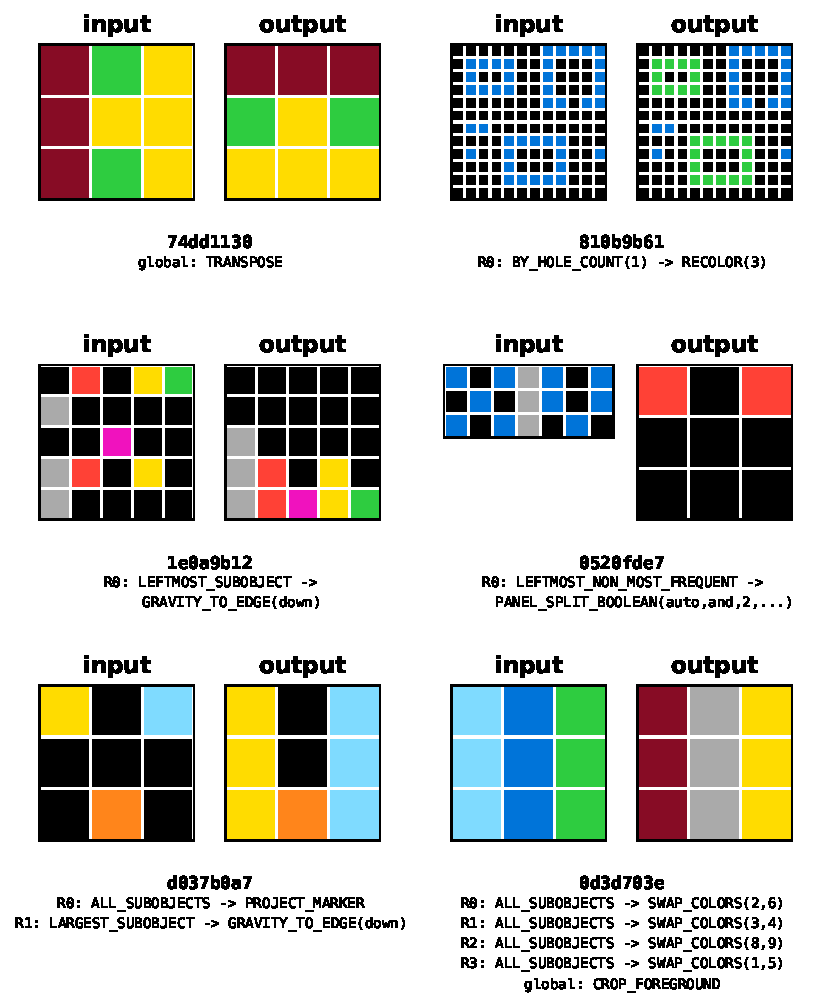
\includegraphics[width=0.95\textwidth]{images/thesis/thesis-fig-gallery.pdf}
    \caption{Six solved ARC-AGI-1 training tasks with the programs that solve them, one panel
    each: the withheld test pair, input left and output right, under the task identifier and
    the winning program. Arguments are abbreviated to their values; Table~\ref{tab:app-selargs}
    and Table~\ref{tab:app-actargs} give the names and ranges.}
    \label{fig:app-gallery}
\end{figure}

\paragraph{A resolved task, in full.} Task \texttt{31aa019c}
(Section~\ref{sec:exp-worked}) is a useful worked example because it exercises a parser
toggle, a relational selector, and a geometric action on a readable $10\times10$ grid. The
program the search discovered is two rules and an identity global transform:

\begin{quote}
\ttfamily
Rule 0:\quad LEAST\_FREQUENT\_COLOR\_OBJECTS() $\to$ KEEP\_SELECTED()\\
Rule 1:\quad REFERENCE\_SINGLETONS() $\to$ STAMP\_LOCAL\_PATTERN(\\
\hspace*{3em}pattern=ring, anchor=centroid, color\_source=self)\\
Global:\quad IDENTITY
\end{quote}

\noindent The first rule keeps the objects of the rarest colour and drops the rest; the
second finds the single-cell reference objects that survive and stamps a ring around each,
taking the ring's colour from the object itself. Nothing in the program names a specific
colour or coordinate: the ``rarest colour'' is resolved per task, and the ring colour is
copied from whatever object the rule lands on, which is why the same two rules generalize
across the task's train and test pairs.

\section{Operator arguments}
\label{app:opargs}

Most selectors and actions take arguments, drawn per task by the codec's samplers at
genome-construction time. Table~\ref{tab:app-selargs} and Table~\ref{tab:app-actargs} give
the argument names and their legal ranges for the most frequently used operators; the full
set follows the same pattern. Numeric ranges are inclusive. Colours are grid colours
$0$--$9$, and a colour argument is drawn from the task's output-colour prior most of the
time and uniformly otherwise, so the search stays global while favouring plausible colours.

\begin{table}[htbp]
\centering
\caption{Arguments of representative selectors.}
\label{tab:app-selargs}
\small
\begin{tabular}{p{4.6cm}p{8.4cm}}
\hline\noalign{\smallskip}
Selector & Arguments \\
\noalign{\smallskip}\hline\noalign{\smallskip}
\texttt{BY\_COLOR} & \texttt{color} $\in [0,9]$ \\
\texttt{BY\_MASS\_AT\_LEAST} & \texttt{mass} $\in [1,9]$ \\
\texttt{BY\_MASS\_EXACT} & \texttt{mass} $\in [1,9]$ \\
\texttt{BY\_HOLE\_COUNT} & \texttt{holes} $\in \{0,1,2,3,4\}$ \\
\texttt{HAS\_EDGE\_TYPE} & \texttt{edge\_type} (one of the edge types); \texttt{direction} $\in \{$outgoing, incoming, both$\}$ \\
\texttt{NEAREST\_TO\_SELECTOR} & \texttt{distance} $\in \{$centroid, bbox\_gap$\}$; \texttt{top\_k} $\in [1,4]$; \texttt{include\_references} $\in \{$true, false$\}$ \\
\texttt{BY\_NOISE\_SCORE} & \texttt{min\_score}, \texttt{max\_score} $\in [0,1]$; \texttt{order} $\in \{$none, highest, lowest$\}$; \texttt{top\_k} $\in [1,4]$ \\
\texttt{SELECTOR\_SET\_OP} & \texttt{op} $\in \{$intersection, difference, union$\}$; nested left/right selector kinds and their arguments \\
\noalign{\smallskip}\hline
\end{tabular}
\end{table}

\begin{table}[htbp]
\centering
\caption{Arguments of representative actions.}
\label{tab:app-actargs}
\small
\begin{tabular}{p{4.6cm}p{8.4cm}}
\hline\noalign{\smallskip}
Action & Arguments \\
\noalign{\smallskip}\hline\noalign{\smallskip}
\texttt{RECOLOR} & \texttt{color} $\in [0,9]$ (output-colour prior) \\
\texttt{TRANSLATE} & \texttt{dy}, \texttt{dx} $\in [-10,10]$ \\
\texttt{TRANSLATE\_WRAP} & \texttt{dy}, \texttt{dx} $\in [-10,10]$, wrapping at the edges \\
\texttt{COPY\_TRANSLATE} & \texttt{dy}, \texttt{dx} $\in [-10,10]$ \\
\texttt{DILATE\_SELECTED} & \texttt{radius} $\in \{1,2\}$; \texttt{connectivity} $\in \{4,8\}$; \texttt{mask} $\in \{$auto, cross, diamond, square$\}$ \\
\texttt{RECOLOR\_SEQUENCE} & \texttt{order} $\in \{$y\_then\_x, x\_then\_y, mass\_desc, mass\_asc$\}$; \texttt{start\_color} $\in [0,9]$; \texttt{step} $\in \{1,2,3\}$ \\
\texttt{SWAP\_COLORS} & \texttt{color\_a}, \texttt{color\_b} $\in [0,9]$, \texttt{color\_a} $\ne$ \texttt{color\_b} \\
\texttt{STAMP\_LOCAL\_PATTERN} & \texttt{pattern} $\in \{$dot, cross, x, ring, square$\}$; \texttt{anchor} $\in \{$centroid, bbox\_center, min\_corner$\}$; \texttt{color\_source} $\in \{$self, constant, background$\}$; \texttt{color} $\in [0,9]$ \\
\texttt{EXTEND\_LINE\_UNTIL} & \texttt{direction} (one of twelve); \texttt{stop\_condition} $\in \{$boundary, touch\_object, non-background$\}$; \texttt{color}, \texttt{intersection\_color} $\in [0,9]$ \\
\texttt{RECOLOR\_FROM\_REFERENCE} & \texttt{reference\_selector\_kind}; \texttt{color\_policy} $\in \{$nearest, majority, only$\}$; \texttt{match\_policy} $\in \{$same\_shape, same\_shape\_strict, any$\}$ \\
\noalign{\smallskip}\hline
\end{tabular}
\end{table}

\section{The highest-support macros}
\label{app:macrotable}

Table~\ref{tab:app-macros} lists the ten highest-support macros of the deployment library
(116 macros mined from 335 solved tasks and 1069 programs;
Section~\ref{sec:macros}). Each row gives the role skeleton, the dominant concrete
head per slot, and the support, meaning the number of distinct tasks the skeleton was mined
from. The list reads as a census of the recurring two-rule strategies in the solved set:
paired colour-class moves, paired size-keyed recolourings, relational recolour chains, and
projection pairs. Most of the top macros are role-level with no cross-slot binding; the
coupled ``same colour in both rules'' macros, which the reachability analysis
(Section~\ref{sec:macros}) identifies as the ones a plain sampler rarely
reaches, appear a little lower in the ranking, the strongest carrying a colour binding at
fraction $0.75$.

\begin{table}[htbp]
\centering
\caption{The ten highest-support macros of the deployment library. ``Head'' is the
top concrete \texttt{(selector, action)} pair for each slot; support is the number of
distinct source tasks.}
\label{tab:app-macros}
\footnotesize
\begin{tabular}{p{2.0cm}p{7.4cm}r}
\hline\noalign{\smallskip}
Skeleton & Dominant heads (slot 1; slot 2) & Support \\
\noalign{\smallskip}\hline\noalign{\smallskip}
COLORCLASS, MOVE $\times2$ & \texttt{by\_color$\to$translate\_wrap}; same & 18 \\
RELATIONAL, RECOLOR $\times2$ & \texttt{nearest\_to\_selector$\to$recolor\_sequence}; same & 17 \\
SIZE, RECOLOR $\times2$ & \texttt{by\_mass\_exact$\to$recolor}; same & 17 \\
COLORCLASS, RECOLOR $\times2$ & \texttt{least\_frequent\_color\_objects$\to$recolor}; same & 15 \\
COLORCLASS, PROJECT $\times2$ & \texttt{by\_color$\to$stamp\_local\_pattern}; same & 14 \\
PICK1, RECOLOR; COLORCLASS, RECOLOR & \texttt{rightmost\_subobject$\to$recolor\_sequence}; \texttt{most\_frequent\_color\_objects$\to$recolor} & 13 \\
PICK1, RECOLOR $\times2$ & \texttt{smallest\_subobject$\to$recolor}; \texttt{largest\_subobject$\to$recolor} & 12 \\
ALL, PROJECT $\times2$ & \texttt{all\_subobjects$\to$stamp\_local\_pattern}; same & 11 \\
COLORCLASS, RECOLOR; RELATIONAL, RECOLOR & \texttt{by\_color$\to$recolor}; \texttt{farthest\_from\_selector$\to$recolor} & 11 \\
COLORCLASS, RECOLOR; PICK1, RECOLOR & \texttt{most\_frequent\_color\_objects$\to$recolor}; \texttt{smallest\_subobject$\to$recolor} & 9 \\
\noalign{\smallskip}\hline
\end{tabular}
\end{table}

\chapter{Notation and Abbreviations}
\label{app:notation}

This appendix collects the symbols and abbreviations used throughout the thesis, for
reference. Table~\ref{tab:app-notation} lists the mathematical notation and
Table~\ref{tab:app-abbrev} the abbreviations.

\begin{table}[htbp]
\centering
\caption{Notation.}
\label{tab:app-notation}
\small
\begin{tabular}{p{2.6cm}p{10.4cm}}
\hline\noalign{\smallskip}
Symbol & Meaning \\
\noalign{\smallskip}\hline\noalign{\smallskip}
$I$ & an individual, the triple $(\mathcal{I}, \mathcal{P}, \mathcal{O})$ \\
$\mathcal{I}$ & a parser configuration (a \texttt{GraphConfig}) \\
$\mathcal{P}$ & a program (a list of rules plus an optional global transform) \\
$\mathcal{O}$ & a projector configuration \\
$G_{\mathrm{in}}$ & the input graph, the parsing of an input grid \\
$G_{\mathrm{out}}$ & the output graph after the program rewrites $G_{\mathrm{in}}$ \\
$(y, x)$ & the coordinate convention throughout: row then column \\
$O_t$ & a target (ground-truth) output grid \\
$\bar{O}$ & a predicted output grid \\
$c$ & a grid colour, an integer in $[0, 9]$ \\
$K$ & the elite count carried between generations \\
$N$ & the seed top-$N$ macro count \\
$\varepsilon$ & the tolerance band of $\varepsilon$-lexicase selection \\
\noalign{\smallskip}\hline
\end{tabular}
\end{table}

\begin{table}[htbp]
\centering
\caption{Abbreviations.}
\label{tab:app-abbrev}
\small
\begin{tabular}{p{2.6cm}p{10.4cm}}
\hline\noalign{\smallskip}
Abbreviation & Expansion \\
\noalign{\smallskip}\hline\noalign{\smallskip}
AGI & artificial general intelligence \\
ARC & Abstraction and Reasoning Corpus \\
ARC-AGI & the renamed ARC benchmark and its versioned successors \\
AST & abstract syntax tree \\
DSL & domain-specific language \\
EC & evolutionary computation \\
GA & genetic algorithm \\
GP & genetic programming \\
IoU & intersection over union \\
LLM & large language model \\
LRM & large reasoning model \\
LOO & leave-one-out \\
MDL & minimum description length \\
SyGuS & syntax-guided synthesis \\
\noalign{\smallskip}\hline
\end{tabular}
\end{table}
